\documentclass[t]{beamer}

% Load general definitions
% Preamble file - general definitions, package loading, etc.

%=================================
% Load packages
\usepackage{amssymb,amsmath}
\usepackage{graphicx}
\usepackage{url}
\usepackage{tikz}
\usetikzlibrary{mindmap,trees,arrows}
\usepackage{fancyvrb}
\usepackage[portuguese]{babel} 
\usepackage[utf8]{inputenc}
\usepackage{subfigure}
\usepackage{times}
\usepackage[T1]{fontenc}
\usepackage{cancel}
\usepackage{color}
\usepackage{listings}
\usepackage[document]{ragged2e}

%=================================
% Set mode
\mode<presentation>
{
	\usetheme{Madrid}
	\usecolortheme{structure}
	\useoutertheme{infolines}
	\setbeamercovered{invisible}
}

% Get rid of nav bar
\beamertemplatenavigationsymbolsempty

% Insert frame number at bottom of the page.
\usefoottemplate{\hfil\tiny{\color{black!90}\insertframenumber}} 

%=================================
% Define new commands

\newcommand\Real{{\mathbb{R}}}
%\newcommand{\vi}{\vspace{0.6\baselineskip}}
%\newcommand{\goodgap}{\hspace{\subfigtopskip}\hspace{\subfigbottomskip}}


% Equation environments
\newcommand{\beq}{\begin{equation}}
\newcommand{\eq}{\end{equation}}
\newcommand{\beqs}{\begin{equation*}}
\newcommand{\eqs}{\end{equation*}}
\newcommand{\beqn}{\begin{eqnarray}}
\newcommand{\eqn}{\end{eqnarray}}
% Bold variables
\newcommand{\mbf}[1]{\ensuremath{\mathbf{#1}}}
% Itemization
\newcommand{\bitem}{\begin{itemize}}
\newcommand{\eitem}{\end{itemize}}
\newcommand{\spitem}{\vskip 1em\item}
\newcommand{\bitems}{\begin{itemize}\item}
\newcommand{\benums}{\begin{enumerate}\item}
\newcommand{\eenum}{\end{enumerate}}
% color blocks
\newenvironment{colorblock}[2]{%
\setbeamercolor{block title}{#2}
\begin{block}{#1}}{\end{block}}
% Vertical spacing
\newcommand{\vone}{\vskip 1em}
\newcommand{\vhalf}{\vskip .5em}
% Frame environments
\newenvironment{ftst}[3][t]{%
\begin{frame}{environment=ftst,#1}
\frametitle{#2}
\framesubtitle{#3}}{\end{frame}}
\newenvironment{ftstf}[2]{
\begin{frame}[fragile,environment=ftstf]
\frametitle{#1}
\framesubtitle{#2}}{\end{frame}}
% colors
\definecolor{MyGray}{rgb}{0.5,0.5,0.5}
\definecolor{MyDBGray}{rgb}{0.1,0.1,0.4}
\definecolor{darkgreen}{rgb}{0,0.4,0}
\definecolor{black}{rgb}{0,0,0}
\def\defn#1{{\color{red} #1}}
% Footnote
\renewcommand{\thefootnote}{\alph{footnote}}
% Relaxed footnotes
\newcommand{\lfr}[1]{\let\thefootnote\relax\footnote{\tiny #1}}
% Verbatim environment - using FANCYVRB package
\DefineVerbatimEnvironment%
{rcode}{Verbatim}
{fontsize=\scriptsize}
% Verbatim environment - using LISTINGS package
%\lstnewenvironment{rcode} {\lstset{	language = R,
%									basicstyle = \scriptsize\ttfamily,
%									showspaces = false,
%									showstringspaces = false,
%									showtabs = false,
%									keywordstyle = \color{black}\bfseries,
%									commentstyle = \color{darkgreen},
%									numbers = none,
%									otherkeywords={	<-,
%													ggplot,
%													geom_boxplot,
%													facet_grid,
%													shapiro.test,
%													fligner.test,
%													glht,
%													with},
%									deletekeywords={data,
%													model,
%													residuals,
%													c,
%													axis,
%													default,
%													labels,
%													qq.text}}}%
%{}

% Specific definitions
\title[]{Metodologia Científica}
\subtitle[]{Redação Científica - Introdução}
\author[]{Patrícia Lucas\\{\footnotesize }}
\institute{Bacharelado em Sistemas de Informação \\ IFNMG  - Campus Salinas}
\date{\scriptsize Salinas\\Junho 2021}

\begin{document}

% cover page
\setbeamertemplate{footline}{}
\begin{frame}

\begin{center}
\includegraphics[width=.15\textwidth]{}
\end{center}
  \titlepage
  \begin{tikzpicture}[remember picture,overlay]
  \node[anchor=south east,xshift=-5pt,yshift=5pt] at (current page.south east) {\tiny Versão 1.2021};
  \node[anchor=south west,yshift=0pt] at (current page.south west) {
\includegraphics[width=.25\textwidth]{Logos/salinas_horizontal_jpg.jpg}};
  \end{tikzpicture}  
\end{frame}

% Main slides

\begin{ftst}{Referência}{Redação Científica}

\justifying
\begin{figure}
    \centering
    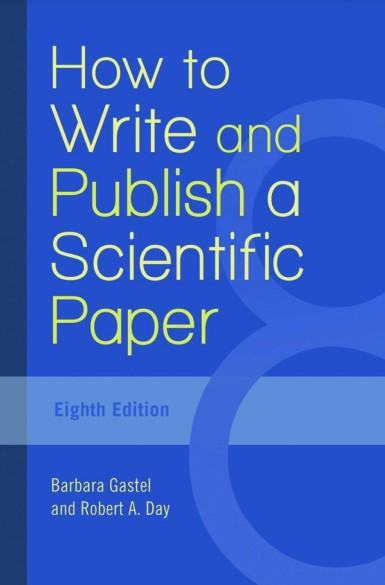
\includegraphics[scale=0.35]{Figuras/ref2.jpg}
\end{figure}

Gastel, Barbara; Day, Robert A. How to Write and Publish a Scientific Paper. Califórnia: Greenwood, 2016.

\end{ftst}

%=====


\begin{ftst}{O escopo}{Redação Científica}
\justifying
O termo redação científica comumente inclui:
\vone
\begin{itemize}
    \item o relato de pesquisas originais em periódicos, por meio de artigos científicos em formato padrão.
    \item a comunicação sobre ciência por meio de outros tipos de artigos de periódicos, como artigos de revisão que resumem e integram pesquisas publicadas anteriormente.
    \item em um sentido ainda mais amplo, outros tipos de comunicação profissional por cientistas - por exemplo, propostas de bolsas, apresentações orais e apresentações de pôsteres.
\end{itemize}


\end{ftst}

%=====

\begin{ftst}{A necessidade de clareza}{Redação Científica}
\justifying
\textbf{A principal característica da redação científica é a clareza.}
\vone
A experimentação científica bem-sucedida é o resultado de uma mente clara atacando um problema claramente declarado e produzindo conclusões claramente definidas.
\vone
Idealmente, a clareza deve ser uma característica de qualquer tipo de comunicação; entretanto, quando algo está sendo dito pela primeira vez, clareza é essencial.
\vone
A maioria dos artigos científicos são aceitos para publicação precisamente porque contribuem com novos conhecimentos. Portanto, \textcolor{blue}{a clareza absoluta é uma exigência na redação científica}.

\end{ftst}

%=====


\begin{ftst}{Recebendo os sinais}{Redação Científica}
\justifying
Se uma árvore cai na floresta e não há ninguém para ouvi-la cair, ela faz algum barulho?
\vone
A resposta correta é não. O som é mais do que ondas de pressão e, de fato, não pode haver som sem um ouvinte.
\vone
Assim como um sinal de qualquer tipo é inútil a menos que seja percebido, um artigo científico publicado (sinal) é inútil a menos que seja recebido e compreendido por seu público-alvo.
\vone
\textbf{Conclusão:} um experimento científico não está completo até que os resultados tenham sido publicados e compreendidos.
\vone
Muitos artigos científicos caem silenciosamente na floresta!

\end{ftst}

%=====

\begin{ftst}{Entendendo os sinais}{Redação Científica}
\justifying
A escrita científica é a transmissão de um sinal claro a um destinatário. As palavras do sinal devem ser o mais claras, simples e bem ordenadas possível.
\vone
Na redação científica, há pouca necessidade de ornamentação. Enfeites literários floridos - metáforas, símiles, expressões idiomáticas - podem causar confusão e raramente devem ser usados em trabalhos de pesquisa.
\vone
A ciência é simplesmente importante demais para ser comunicada em qualquer outra coisa senão em palavras de significado certo. 
\vone
Muitos tipos de escrita são projetados para entretenimento. \textbf{A escrita científica tem um propósito diferente: comunicar novas descobertas científicas.}



\end{ftst}

%=====

\begin{ftst}{Entendendo o contexto}{Redação Científica}
\justifying
O que é claro para um destinatário depende tanto do que é transmitido quanto de como o destinatário o interpreta.
\vone
Portanto, comunicar-se claramente requer consciência do que o destinatário traz. Qual é o histórico do destinatário? O que o destinatário está procurando? Como o destinatário espera que a redação seja organizada? Clareza na redação científica requer atenção a tais questões.
\vone
Conheça o seu público! Conheça também as convenções e, portanto, as expectativas para estruturar o tipo de redação que você está fazendo.



\end{ftst}

%=====

\begin{ftst}{Organização e linguagem}{Redação Científica}
\justifying
Uma organização eficaz é a chave para se comunicar de forma clara e eficiente em ciência. 
\vone
Essa organização inclui seguir o formato padrão de um artigo científico. Também inclui organizar ideias de forma lógica dentro desse formato. 
\vone
Além da organização, o segundo ingrediente principal de um artigo científico deve ser a linguagem apropriada.
\vone
Dado que o resultado final da pesquisa científica é a publicação, é surpreendente que muitos cientistas negligenciem as responsabilidades envolvidas. 

\end{ftst}

%=====

\begin{ftst}{Organização e linguagem}{Redação Científica}
\justifying
Um cientista gastará meses ou anos de trabalho árduo e, então, despreocupadamente, permitirá que muito de seu valor seja perdido devido à falta de interesse no processo de comunicação.

\vone
Dispositivos literários, metáforas e coisas semelhantes, desviam a atenção da substância para o estilo. Eles devem ser usados raramente em redação científica.

\end{ftst}


\end{document}